% Reference https://www.youtube.com/watch?v=Boltwen-g1g&ab_channel=ChandraHas

\documentclass[11pt,a4paper]{article}

% General
\usepackage[margin=1in]{geometry}
\usepackage[sort&compress,square,numbers]{natbib}
\usepackage{amsmath}
\usepackage{lipsum,times,graphicx,hyperref,cleveref}
\hypersetup{nolinks=true}
\usepackage[labelfont=bf]{caption}
\usepackage{amssymb}

\usepackage{physics}
\usepackage{siunitx}
\usepackage{listings}

% More graphics
\usepackage[label font={bf, normalsize}]{subfig}
\renewcommand{\thesubfigure}{\Alph{subfigure}}
\usepackage{caption}
\captionsetup{font=normal}
\usepackage{floatrow}
\floatsetup[figure]{subcapbesideposition=top}
\floatsetup[table]{style=plaintop}

\usepackage{xr}
\externaldocument[main-]{main}
\externaldocument[supp-]{supp}


\usepackage{titling}
\renewcommand\maketitlehooka{\null\mbox{}\vfill}
\renewcommand\maketitlehookd{\vfill\null}

\title{\vspace{-5cm} {Figures for}\\[5mm] 
\textbf{Behavior of weakly adsorbing protein impurities in flow-through ion-exchange chromatography}}
 
\author{Chase E. Herman, Xuankuo Xu, Steven J. Traylor, Sanchayita Ghose, \and Zheng Jian Li, and Abraham M. Lenhoff}

\date{}

%\renewcommand{\figurename}{Fig.}
\renewcommand{\baselinestretch}{1.33} 
%==============================Content=========================
\begin{document}

%\begin{titlingpage}
%\maketitle
%\end{titlingpage}

\begin{figure}[H]
    \centering
    \sidesubfloat[]{\includegraphics[width=0.9\textwidth]%
                    {figure_1a}\label{sfig:10 mg/ml}}
    \\
    \sidesubfloat[]{\includegraphics[width=0.9\textwidth]%
                    {figure_1b}\label{sfig:1 ug/ml}}
    \caption{Illustrative breakthrough profiles for a simulation of solute loading at \protect\subref{sfig:10 mg/ml} 10 mg/ml and \protect\subref{sfig:1 ug/ml} 1 $\mu$g/ml. Lines correspond to simulations with different $K_{eq}$, which increases by 4 orders of magnitude from left to right. Note that $q_{max}$ was fixed at 100 mg/ml of column for all simulations, and the abscissa is on a logarithmic scale. Simulation parameters are summarized in Supplementary Table S1.}
    \label{fig:exploratory breakthrough curves}
\end{figure}


\begin{figure}[bp]
    \centering
    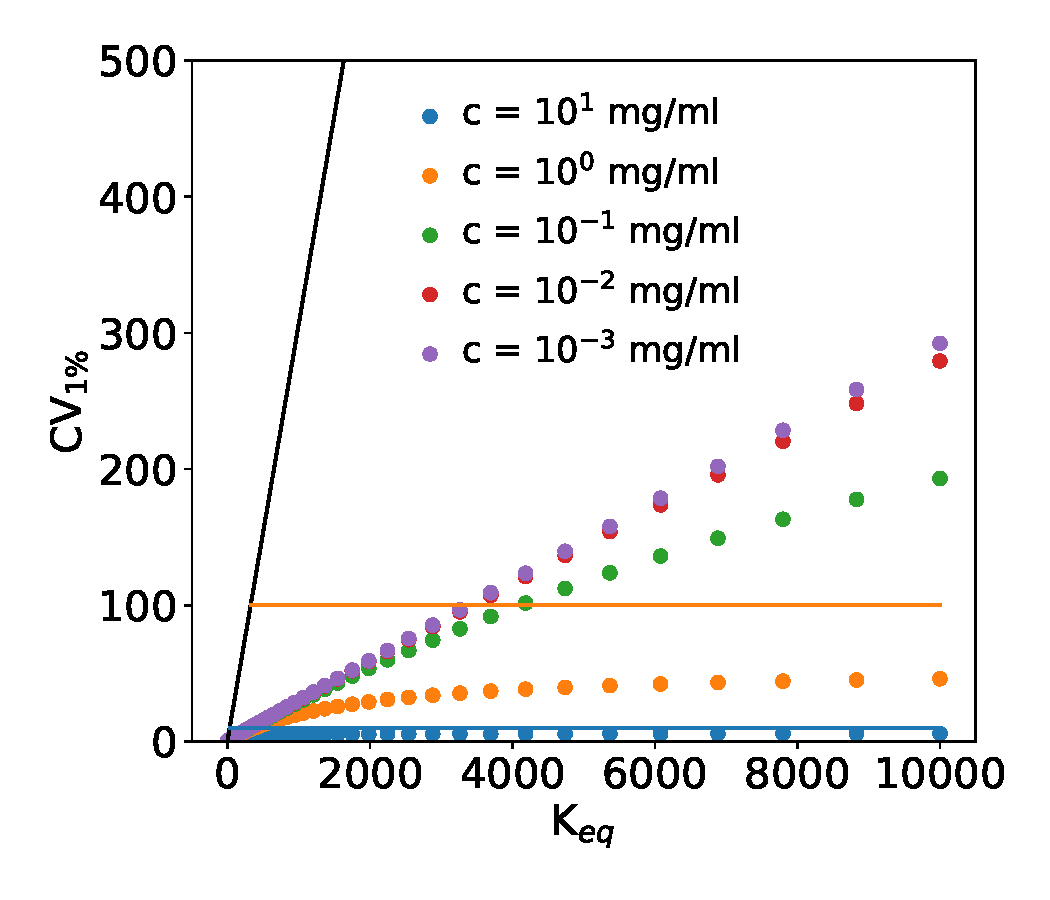
\includegraphics[width=0.9\textwidth]{figure_2}
    \caption{Illustrative dependence of the initial breakthrough volume on $K_{eq}$ and load concentration. $CV_{1\%}$ is the load volume where solute breakthrough reaches 1\%. Horizontal lines represent the hypothetical load volumes required to saturate the column if all of the loaded solute were to adsorb in the absence of transport limitations, which vary with the feed concentration. The solid black line represents the ideal linear limit. Simulation parameters are the same as those in Figure 1.}
    \label{fig:initial breakthrough volumes vs Keq}
\end{figure}


\begin{figure}[bp]
    \centering
    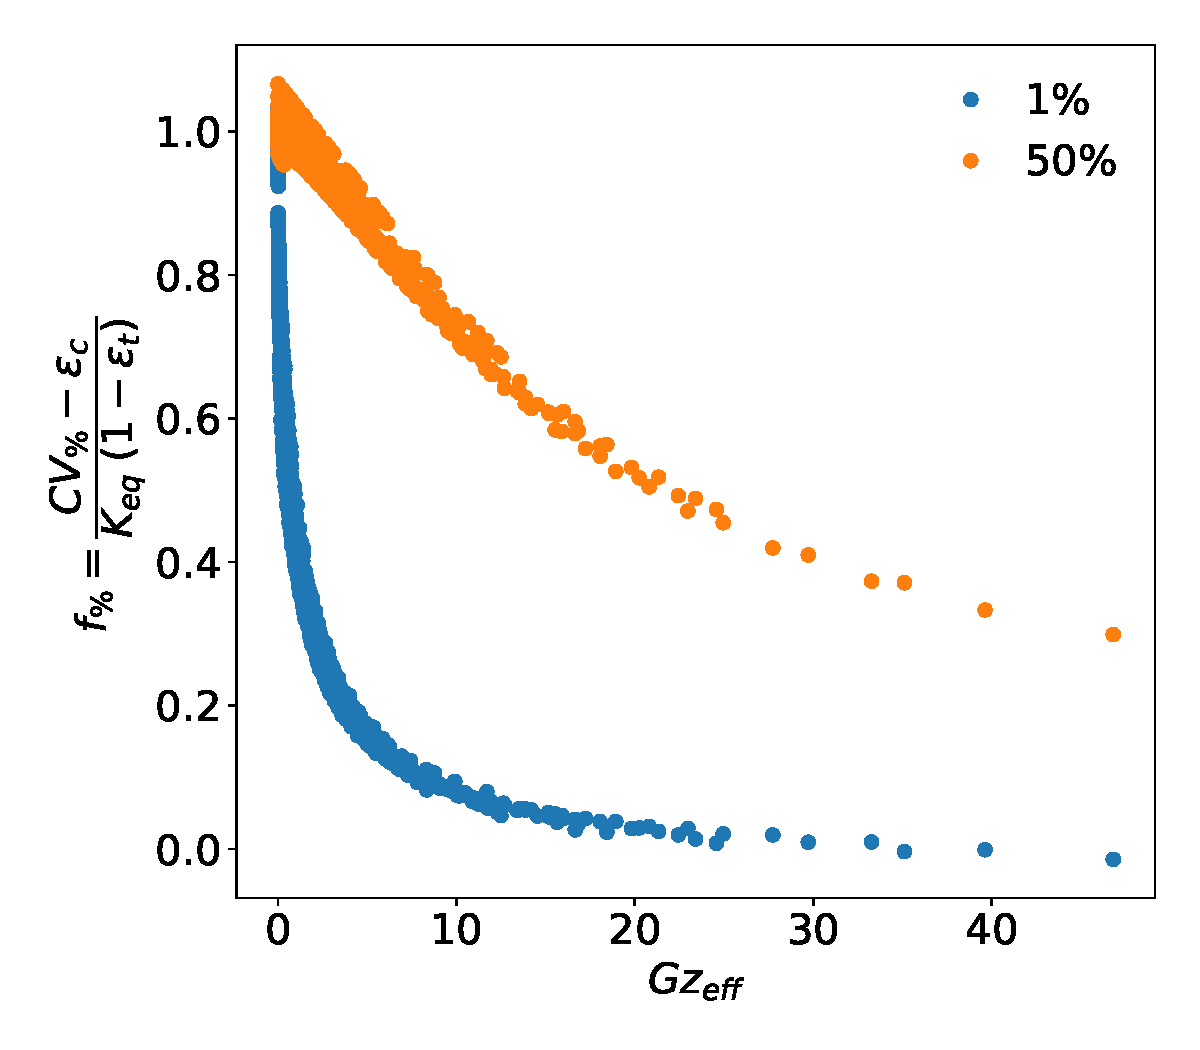
\includegraphics[width=0.9\textwidth]{figure_3}
    \caption{Correlation of breakthrough volumes that were simulated for a 1 $\mu$g/ml feed. The blue and orange series correspond to 1\% and 50\% breakthrough, respectively. Results are shown for simulations with $10 \leq K_{eq} \leq 10000$. Simulation parameters are summarized in Supplementary Table S1.}
    \label{fig:correlation of breakthrough volumes}
\end{figure}


\begin{figure}[bp]
    \centering
    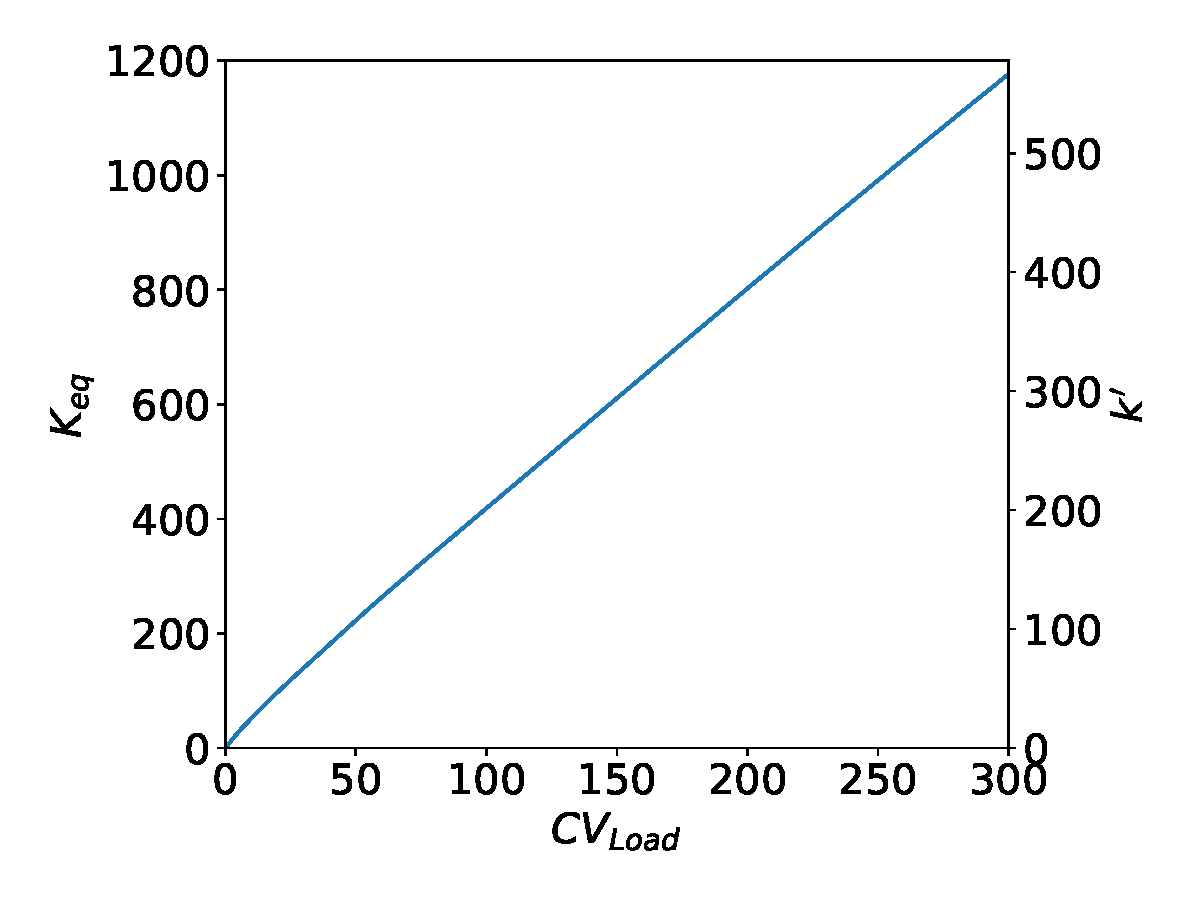
\includegraphics[width=0.8\textwidth]{figure_4}
    \caption{Estimation of potentially problematic $K_{eq}$ as a function of load volume for typical process parameters. Dilute impurities with $K_{eq}$ below the line are expected to break through before the end of loading. Equivalent $k'$ values corresponding to $K_{eq}$ are shown on the right hand axis.}
    \label{fig:problematic Keq}
\end{figure}


\begin{figure}[htbp]
    \centering
    \sidesubfloat[]{\includegraphics[width=0.7\textwidth]%
                    {figure_5a}\label{sfig:100 B}}
    \\
    \sidesubfloat[]{\includegraphics[width=0.7\textwidth]%
                    {figure_5b}\label{sfig:30 B}}
    \caption{Validation of the breakthrough volume correlation with lysozyme on SP Sepharose FF. Breakthrough profiles are shown for \protect\subref{sfig:100 B} non-adsorbing (high ionic strength) conditions and \protect\subref{sfig:30 B} adsorbing (low ionic strength) conditions at different superficial velocities. Solid lines represent experiment, and dashed lines represent simulation. Concentrations were estimated from absorbance profiles at 215 nm.
    %Simulation results are not shown for adsorbing conditions at 30 cm/h due to inaccuracies in describing extra-column effects at low flow rates with the simplified CSTR + PFR model.
    }
    \label{fig:validation with lysozyme}
\end{figure}


\begin{figure}[bp]
    \centering
    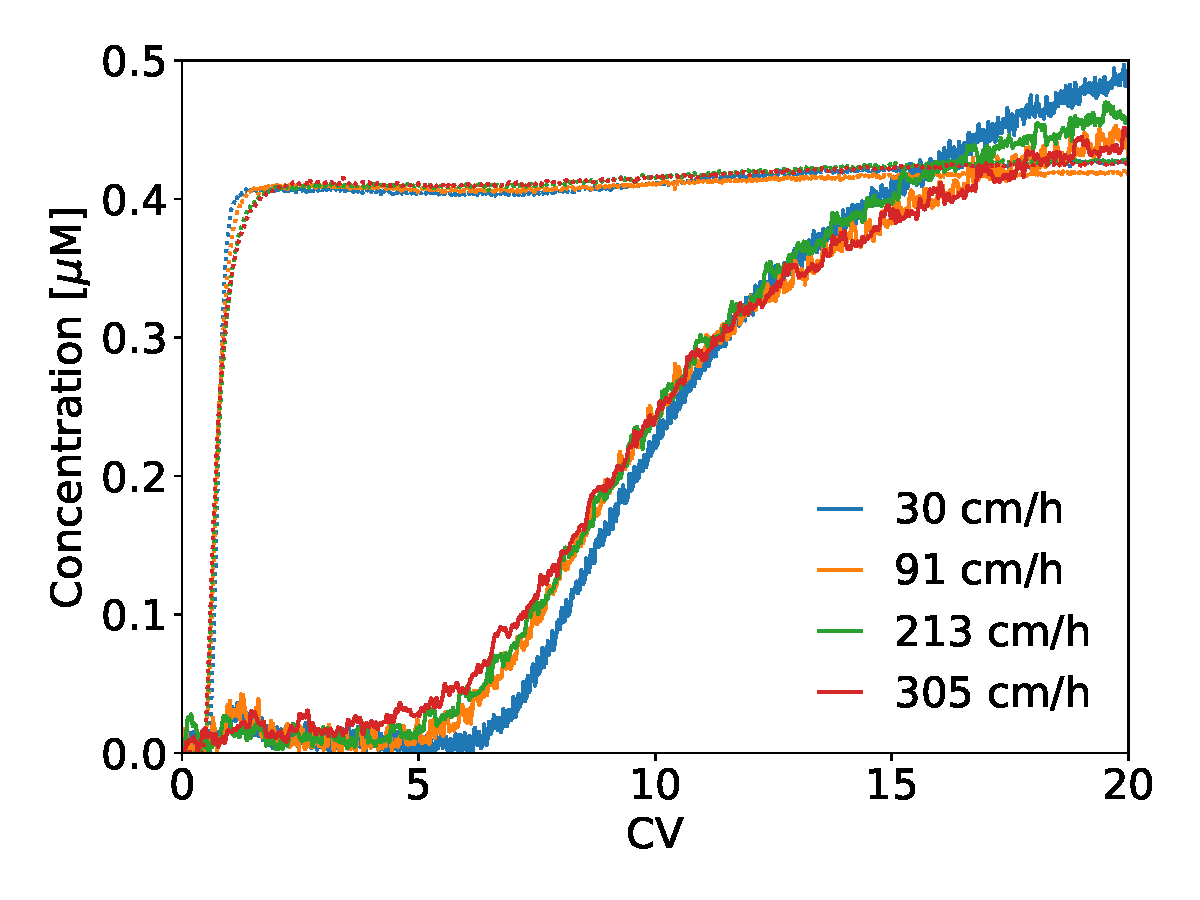
\includegraphics[width=0.9\textwidth]{figure_6}
    \caption{Validation of the breakthrough volume correlation with FITC-lysozyme (solid lines) in the presence of a mAb (dotted lines) at different superficial velocities. Component concentrations were estimated from absorbance profiles at 495 and 280 nm.}
    \label{fig:validation with FITC lysozyme}
\end{figure}


\begin{figure}[htbp]
    \centering
    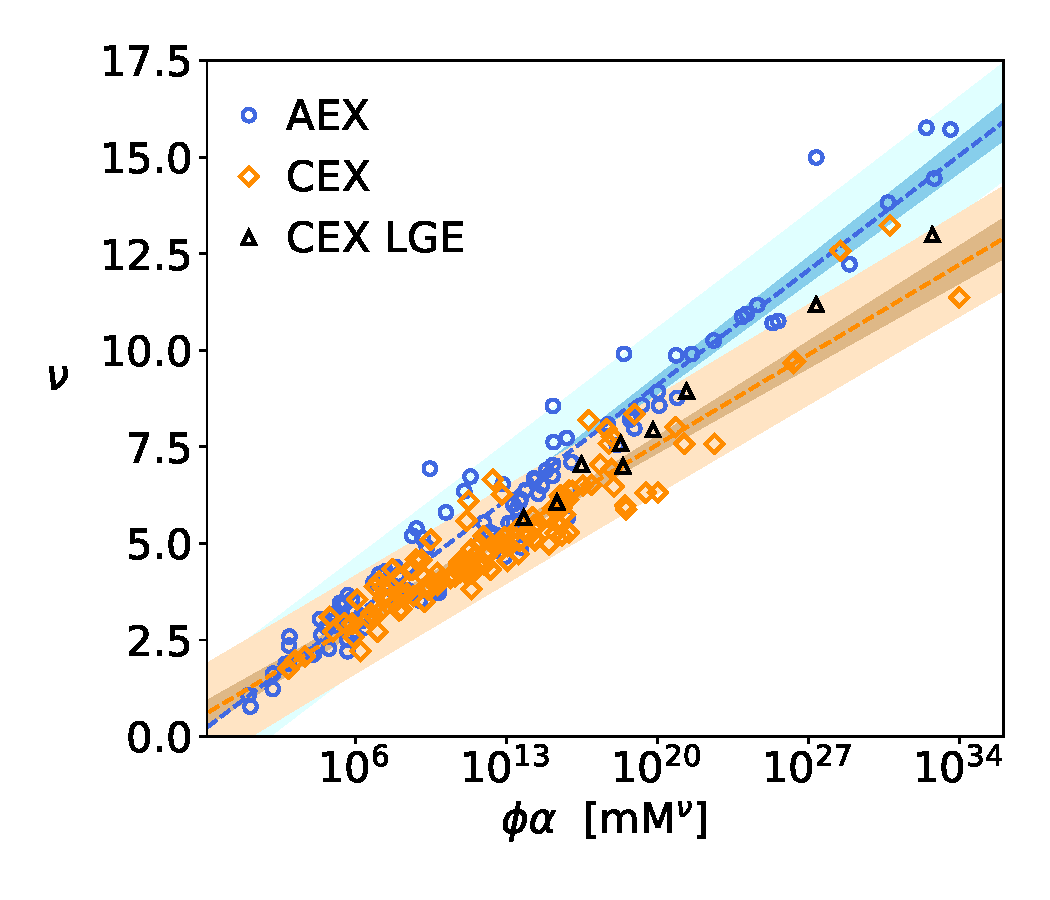
\includegraphics[width=\textwidth]{figure_7}
    \caption{
    Thermodynamic correlation between SDM parameters that were obtained by regressing the consolidated set of isocratic $k'$ data according to Equation~9. Correlation lines for AEX and CEX resins are shown with 95\% confidence intervals (dark shaded regions) and 95\% prediction intervals (light shaded regions). Also shown are parameters that were obtained by regressing linear gradient elution (LGE) data from this work and literature according to Yamamoto's method. Note that the abscissa is on a logarithmic scale.
    }
    \label{fig:sdm parameter correlation}
\end{figure}

\begin{figure}[htbp]
    \centering
    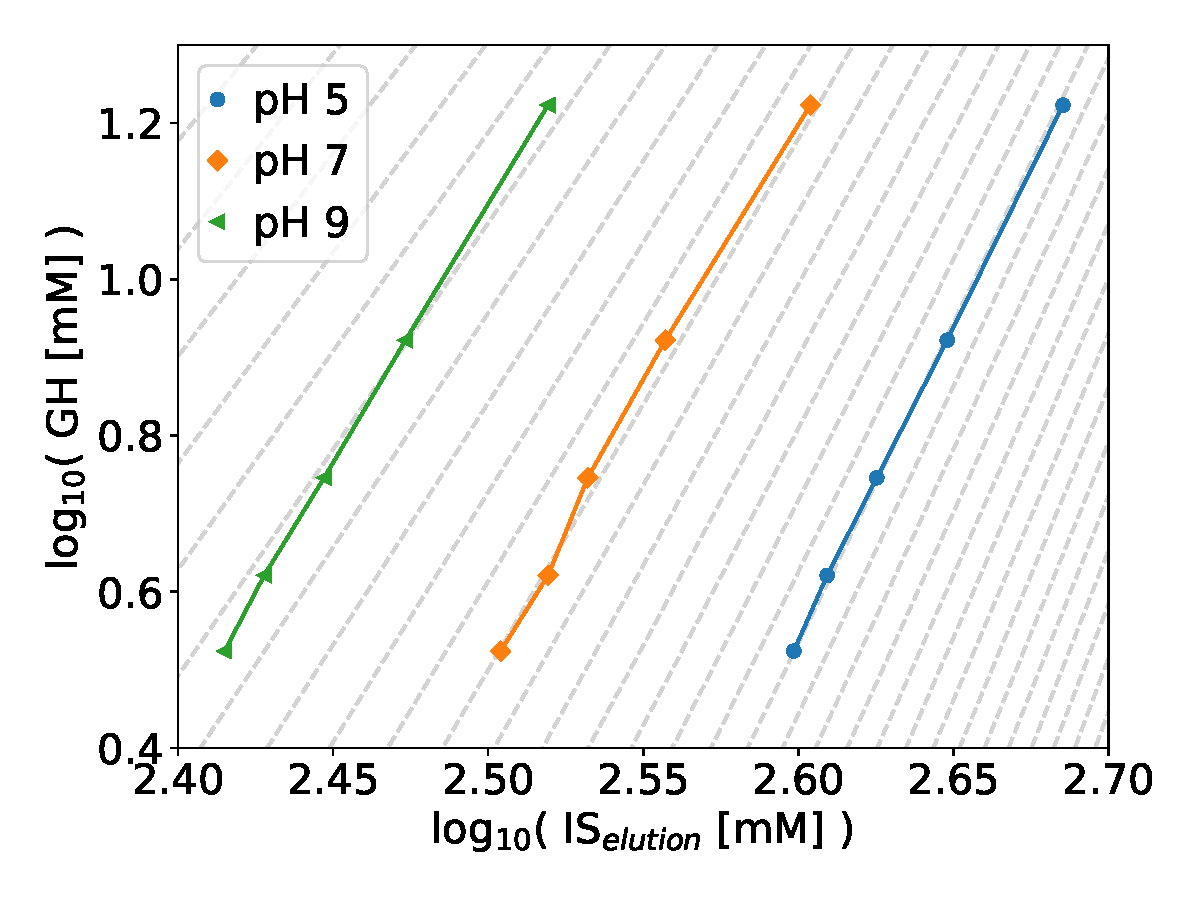
\includegraphics[width=\textwidth]{figure_8}
    \caption{
    Data from the linear gradient elution of lysozyme on SP Sepharose FF plotted in the regression space for Yamamoto's GH analysis method [31]. Dashed grey lines represent predictions based on the SDM parameter correlation for values of $\nu$ that differ by increments of 0.2. For reference, the fit values of ($\nu$, $\alpha$) corresponding to the pH 5, 7, and 9 curves were (7.0, \num{2.2e+19} mM$^{7.0}$), (6.1, \num{1.9e+16} mM$^{6.1}$), and (5.7, \num{5.5e+14} mM$^{5.7}$), respectively, and the values corresponding to the dashed grey lines of closest overlap are (7.2, \num{7.4e19} mM$^{7.2}$), (5.8, \num{4.7e15} mM$^{5.8}$), and (4.8, \num{4.6e12} mM$^{4.8}$), respectively.
    }
    \label{fig:lge overlay}
\end{figure}




\end{document}
